\phantomsection
\label{ch:intro}
\chapter{Introduction}

This chapter presents the main components of this research on Khmer optical character recognition (OCR). It begins with background information on OCR technology and its importance for the Khmer language, followed by identifying the key challenges and research gaps in current Khmer OCR systems. The chapter then outlines the study's objectives and research questions focused on improving Khmer text recognition through synthetic data generation and deep learning approaches. The rationale highlights the significance of developing better OCR tools for preserving and digitizing Khmer texts. Finally, it describes the scope and limitations of the study, along with an overview of the thesis structure.

\section{Background to the Study}
\label{sec:background}


Optical Character Recognition (OCR) technology has become increasingly important in Cambodia's digital transformation journey. As a nation with a rich literary and cultural heritage spanning over a millennium, Cambodia possesses countless historical documents, manuscripts, and texts written in the Khmer script. These materials include ancient palm leaf manuscripts, historical records, educational materials, and government documents that hold significant cultural and practical value.

The Khmer script, which has been in use since the 7th century, presents unique challenges for OCR systems due to its complex writing system. Unlike Latin-based scripts, Khmer is an abugida writing system with intricate character combinations, subscripts, diacritics, and contextual forms. Traditional OCR solutions, which were primarily developed for Latin-based scripts, often struggle with these complexities.

A particularly pressing challenge is the digitization of Khmer educational materials, especially textbooks from grade 1 to grade 12. Many of these essential learning resources exist only in physical form, with their original digital files lost or never created. This creates significant barriers for educators and students who need digital access to these materials for modern learning environments. The lack of digital versions makes it difficult to update, reproduce, or widely distribute these educational resources efficiently.

While some attempts have been made to develop Khmer OCR solutions, most existing systems have limited accuracy and struggle with real-world variations in text appearance, fonts, and document quality. The scarcity of large-scale training datasets for Khmer text recognition has further hampered progress in this field. This situation has created a pressing need for innovative approaches to improve Khmer OCR technology, especially for recovering and digitizing educational materials that are crucial for Cambodia's education system.

In recent years, there has been growing recognition of the need to digitize Khmer texts for preservation, accessibility, and practical applications. Libraries, museums, and educational institutions across Cambodia are increasingly seeking efficient ways to convert physical documents into searchable digital formats. However, the lack of robust Khmer OCR systems has been a significant bottleneck in these digitization efforts, particularly affecting the education sector where digital versions of textbooks are desperately needed.

\begin{table}[ht]
    \caption{Current State of Khmer Textbook Digitization in Cambodia's Education System}
    \vspace{10pt}
    \phantomsection
    \label{sec:textbook}
    \resizebox{\textwidth}{!}{
    \begin{tabular}{|l|l|l|l|}
    \hline
    Education Level & Subject Areas & Format Availability & Notes \\
    \hline
    Grade 1--6 & All core subjects & Mostly physical only & Many original digital files missing \\
    Grade 7--9 & Math, Science, Khmer & Some digital scans & Scanned PDFs, not text-searchable \\
    Grade 10--12 & All major subjects & Few digitized & Hard to find editable versions \\
    \hline
    \end{tabular}
    }
    \end{table}


Beyond the education sector, the need for robust Khmer OCR technology extends to numerous other critical applications across different domains:

\begin{itemize}
    \item \textbf{AI and Language Models:} Digitizing Khmer books and documents from libraries would enable training of large language models on Cambodian content, making AI systems more culturally aware and capable of processing Khmer language queries and knowledge.
    
    \item \textbf{Digital Libraries:} Converting physical books into searchable digital formats would dramatically improve access to knowledge, allowing readers to instantly search across thousands of Khmer texts and enabling advanced research capabilities.
    
    \item \textbf{Cultural Heritage Preservation:} Thousands of ancient palm leaf manuscripts and historical documents in temples and museums require digitization for preservation and scholarly access, while making this knowledge accessible to AI systems for cultural understanding.
    
    \item \textbf{Government Records:} Vast archives of administrative documents, legal records, and civil registries need conversion into machine-readable formats, enabling automated processing and AI-assisted analysis of public records.
    
    \item \textbf{Healthcare Systems:} Medical records and health documentation could be digitized to train specialized medical AI models that understand Khmer medical terminology and practices.
    
    \item \textbf{Business Intelligence:} Companies could extract insights from digitized Khmer business documents using AI analysis, while making their archives searchable and processable by modern business systems.
    
    \item \textbf{Media Archives:} Converting newspapers and magazines into machine-readable text would allow AI systems to analyze decades of cultural and historical information, identifying trends and patterns in Cambodia's social development.
    
    \item \textbf{Research and Academia:} Digitized academic papers and research materials could feed into knowledge bases for AI systems, making Cambodian research more accessible globally while enabling advanced cross-referencing and analysis.
\end{itemize}

These applications highlight how Khmer OCR technology could not only preserve and digitize texts, but also make them machine-readable for AI systems and language models. This would create a powerful feedback loop where better digitization enables smarter AI systems, which in turn can help process and analyze more Khmer content, ultimately making Cambodia's rich textual heritage more accessible and useful in the digital age.


\section{Problem Statement}
\label{sec:problem}

Optical Character Recognition (OCR) for the Khmer language presents a unique set of challenges that significantly hinder the development of accurate and robust recognition systems. Unlike Latin-based scripts, Khmer is an abugida writing system, where each character represents a consonant-vowel unit and includes complex combinations of base characters, subscripts, superscripts, and diacritics. This structural complexity introduces difficulties at both the text detection stage and the text recognition stage.
\begin{figure}[ht]
    \centering
    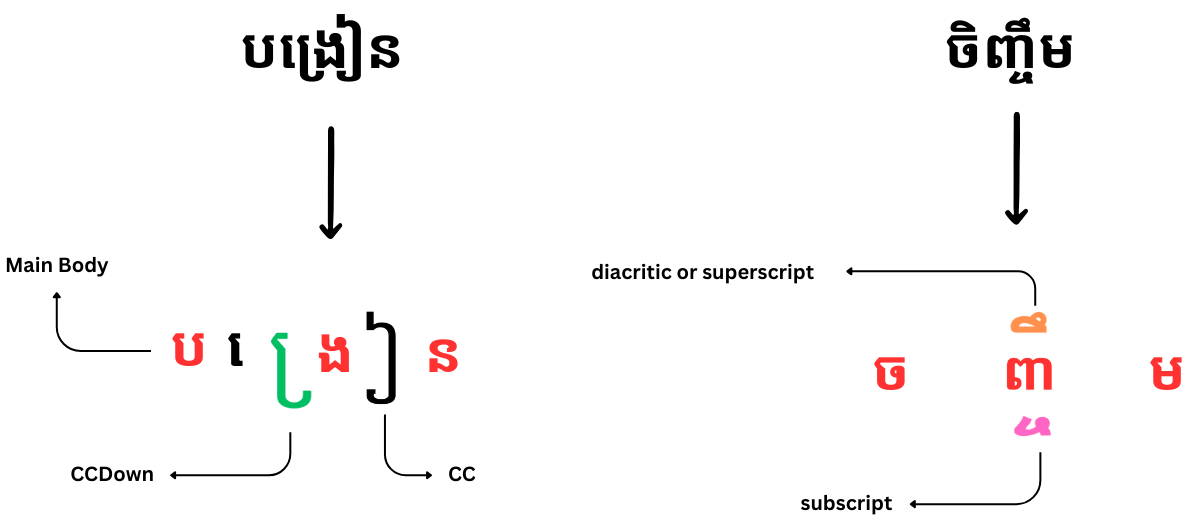
\includegraphics[width=\textwidth]{figures/example_of_text_format.png}
    \caption{Example of Khmer text format showing the complexity of character combinations and diacritics}
    \label{fig:text_format}
\end{figure}

One of the fundamental obstacles is the lack of clear word boundaries in Khmer writing. In contrast to Latin-based languages, where spaces are consistently used to separate words, spaces in Khmer are used infrequently and inconsistently. This makes it extremely difficult to segment text accurately into word-level units for training sequence-to-sequence OCR models such as TrOCR. The absence of reliable word boundaries reduces recognition accuracy and complicates tasks like error correction, search indexing, and language modeling.

\begin{figure}[ht]
    \centering
    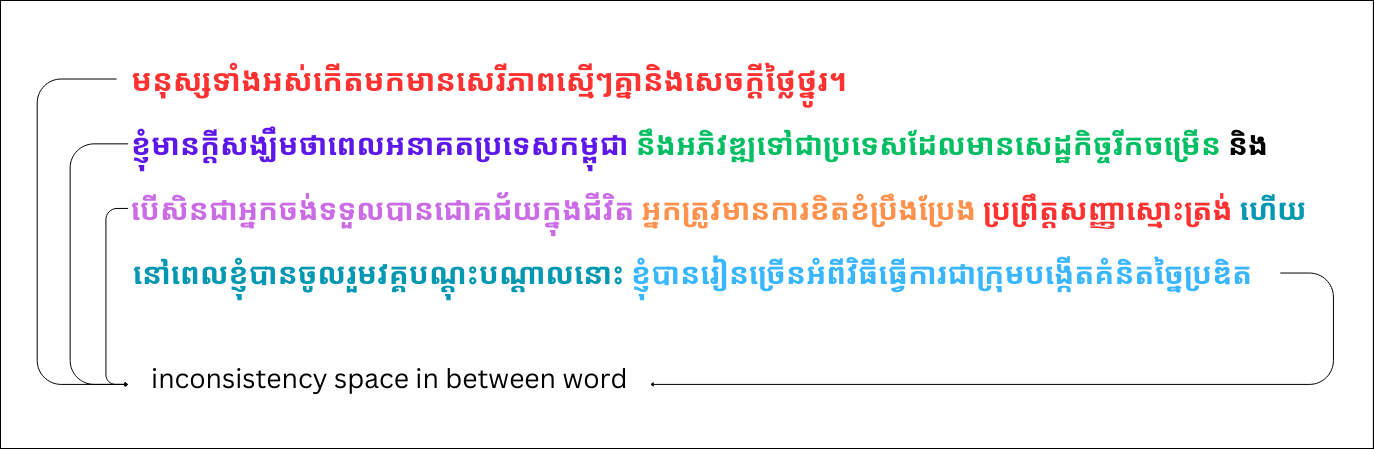
\includegraphics[width=\textwidth]{figures/example_of_long_text.png}
    \caption{Example of sequential Khmer text showing how characters combine to form syllables and words}
    \label{fig:sequential_text}
\end{figure}


A critical barrier to advancing Khmer OCR is the scarcity of annotated training datasets. There is a severe lack of high-quality, large-scale datasets that provide paired image-text data with bounding boxes, character-level annotations, or transcription lines tailored to Khmer script. This data scarcity limits the potential for supervised learning approaches and transfer learning, which are essential for training modern deep OCR models like TrOCR.


Additionally, font and style variability further degrade recognition performance. Khmer documents in the real world are printed in diverse typefaces and stylistic variations (e.g., Khmer OS, Nokora, and Hanuman), with differences in stroke thickness, spacing, and decoration. The lack of standardization across documents and poor documentation of these fonts means that OCR models trained on one style often fail to generalize to others. This problem is exacerbated in noisy or low-resolution scans of textbooks and historical texts.

The challenge of font variability is illustrated in Figure \ref{fig:font_variants}, which shows how the same Khmer text can appear significantly different across various fonts and styles.

\begin{figure}[ht]
    \centering
    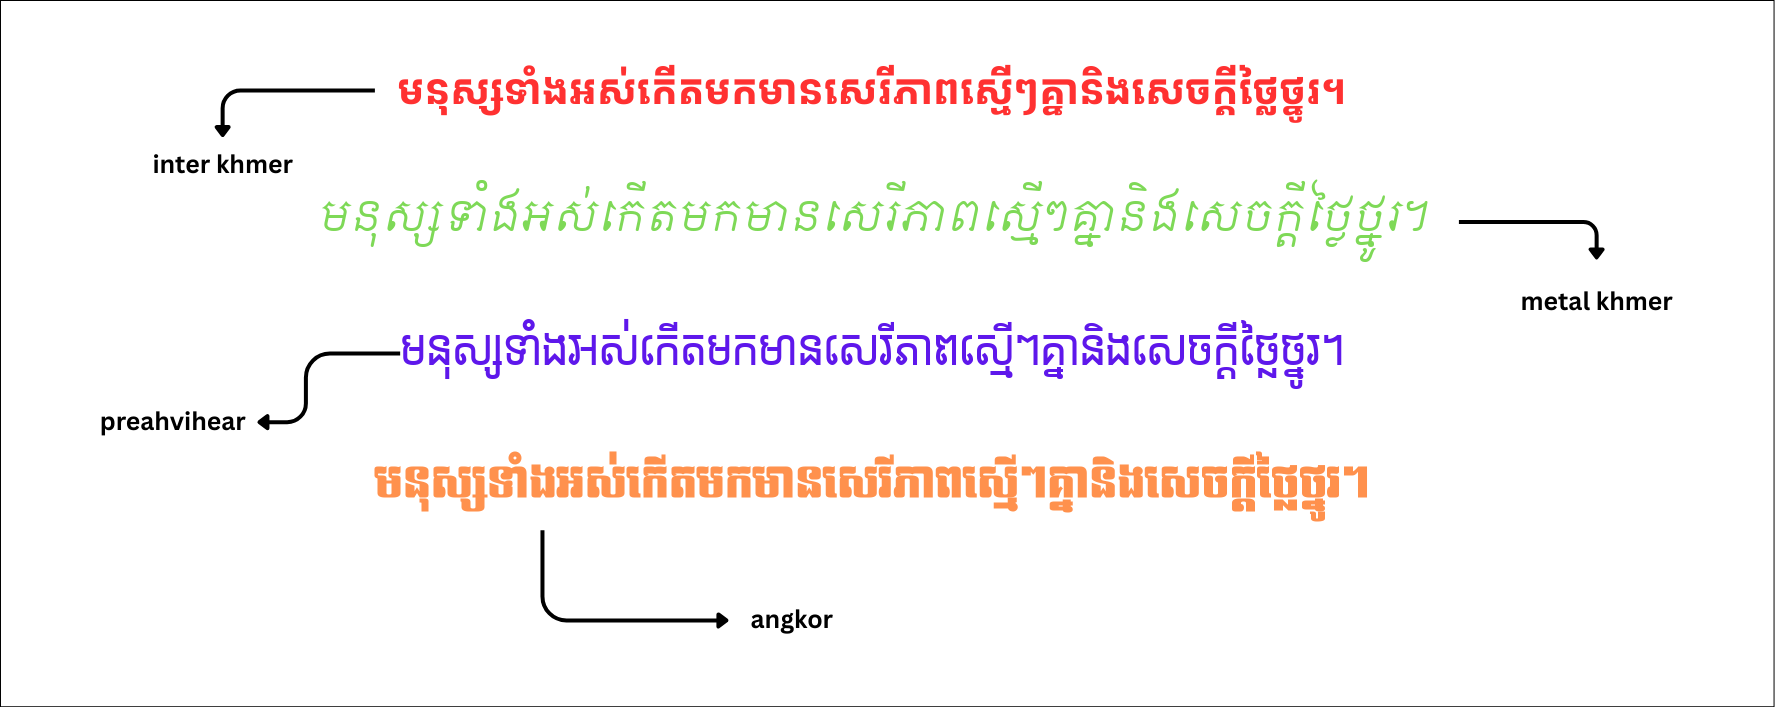
\includegraphics[width=\textwidth]{figures/varianty_of_font.png}
    \caption{Examples of the same Khmer text rendered in different fonts, demonstrating the significant visual variations that OCR systems must handle}
    \label{fig:font_variants}
\end{figure}

\begin{figure}[ht]
    \centering
    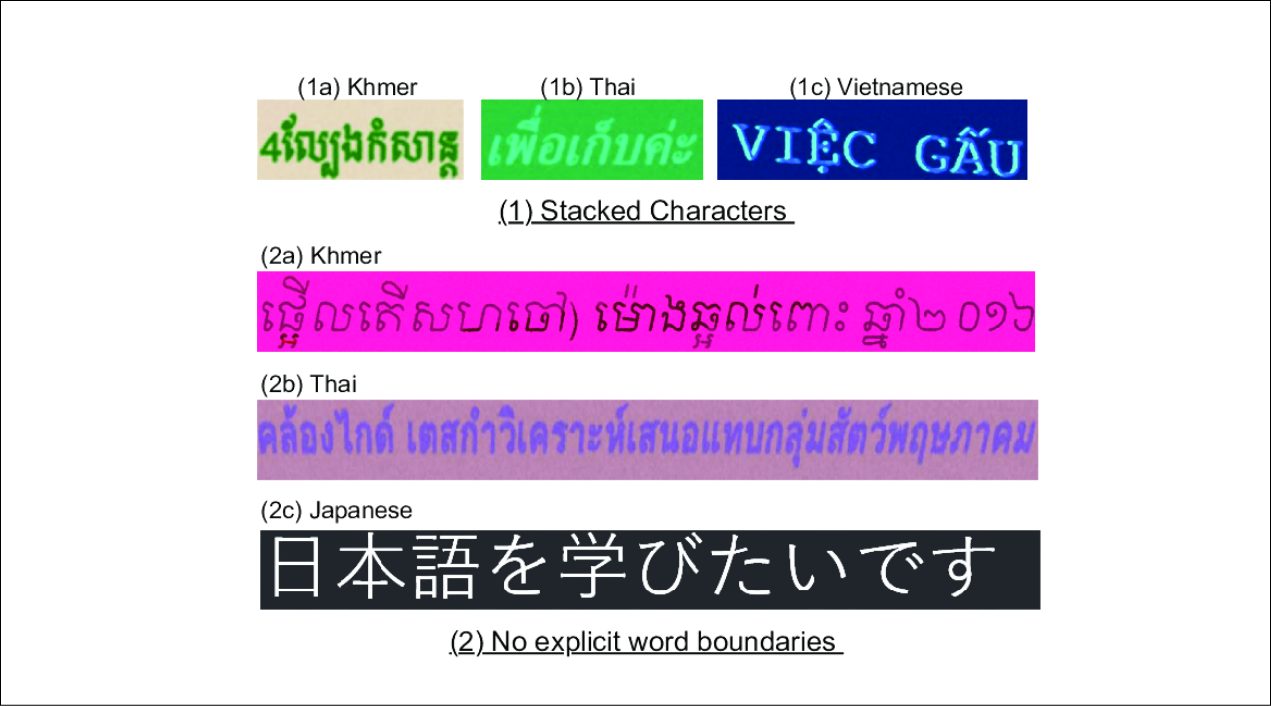
\includegraphics[width=\textwidth]{figures/text_stacking.png}
    \caption{Illustration of Khmer text stacking patterns, showing how characters combine vertically and horizontally to form syllables and words \cite{buoy2023khmerocr}}
    \label{fig:text_stacking}
\end{figure}

Taken together, these challenges create a significant barrier to digitizing Khmer documents using CRAFT + TrOCR pipelines. The absence of word delimiters, the visual complexity of character stacking, cross-script confusion, data scarcity, and font inconsistency all contribute to the low accuracy and poor reliability of existing OCR solutions for Khmer. Addressing these issues requires the development of customized preprocessing, augmentation, and model training strategies—as well as targeted data collection and annotation efforts—to make Khmer OCR viable for real-world applications, especially in the context of educational digitization and cultural preservation.




\section{Aim and Objectives of the Study}
\label{sec:objectives}

The primary aim of this research is to develop an improved optical character recognition (OCR) system specifically designed for MIX-language (Khmer-English) addressing the unique challenges of Khmer-English script while achieving high accuracy and reliability in real-world applications.

The specific objectives of this study are:

\begin{enumerate}
    \item To analyze and quantify the key challenges in Khmer OCR, including character stacking, absence of word boundaries, and font variations
    
    \item To develop enhanced preprocessing techniques that better handle the complex visual structure of Khmer text, particularly focusing on character segmentation and diacritic preservation
    
    \item To create and curate a comprehensive annotated dataset of Khmer text images suitable for training modern OCR models
    
    \item To design and implement customized data augmentation strategies that account for real-world variations in Khmer text appearance
    
    \item To adapt and optimize the CRAFT text detection and TrOCR recognition models for improved performance on Khmer script
    
    \item To evaluate the developed system's performance across different document types, fonts, and quality levels
    
    \item To establish best practices and guidelines for Khmer OCR system development and deployment
\end{enumerate}

Through achieving these objectives, this research aims to significantly advance the state of Khmer OCR technology and enable more effective digitization of Cambodian textual heritage.

\section{Research Questions}
\label{sec:questions}

This research aims to address the following key questions:

\begin{enumerate}
    \item How can text detection and recognition models be effectively adapted to handle the unique characteristics of Khmer script, particularly the stacking of characters and presence of diacritics?
    
    \item What preprocessing and augmentation techniques are most effective for improving OCR accuracy on Khmer text documents with varying fonts, styles, and quality levels?
    
    \item How can the lack of word boundaries in Khmer text be addressed to improve recognition accuracy and enable better post-processing?
    
    \item What are the minimum dataset requirements and optimal annotation strategies for training robust Khmer OCR models?
    
    \item How do different architectural modifications to CRAFT and TrOCR impact recognition performance on Khmer script?
    
    \item What evaluation metrics and benchmarks should be established to meaningfully assess Khmer OCR system performance?
\end{enumerate}

\section{Rationale of the Study}
\label{sec:rationale}
​​​​​  ​ ​ ​  ​ This research is motivated by several compelling factors. First, there is an urgent need to digitize and preserve Cambodia's vast textual heritage, including historical documents, educational materials, and cultural artifacts. Without effective OCR technology for Khmer script, this digitization process remains labor-intensive and prone to errors.

Second, the current limitations of OCR systems for Khmer significantly hinder educational and academic initiatives in Cambodia. Many educational institutions struggle to convert physical textbooks and learning materials into digital formats, impacting accessibility and modernization efforts in education.

Third, the unique challenges posed by Khmer script—from character stacking to the absence of word boundaries—present an opportunity to advance the field of OCR technology as a whole. Solutions developed for Khmer may benefit other scripts with similar characteristics.

Finally, improving Khmer OCR technology aligns with broader digital transformation goals in Cambodia, supporting efforts to preserve cultural heritage while enabling more efficient information processing and accessibility in various sectors.

\section{Limitations and Scope}
\label{sec:limitations}

While this research aims to advance Khmer OCR technology significantly, it is important to acknowledge certain limitations and define the scope of the study:

\begin{enumerate}
    \item The research focuses specifically on printed Khmer text and English text and does not address handwritten text recognition, which presents additional challenges requiring separate investigation.
    
    \item The study primarily considers modern Khmer fonts and typography, with limited coverage of historical or decorative text styles.
    
    \item While the system aims to handle various document quality levels, extremely degraded or damaged documents may fall outside the scope of reliable recognition.
    
    \item The study focuses on optical character recognition and does not extend to higher-level natural language processing tasks such as semantic analysis or machine translation.
    
    \item Resource constraints may limit the size and diversity of the training dataset, though efforts will be made to ensure sufficient representation of common use cases.
\end{enumerate}

These limitations help maintain a focused research scope while acknowledging areas that may require future investigation.

\section{Structure of the Thesis}
\label{sec:structure}

This thesis is organized into the following chapters:

\begin{enumerate}
    \item \textbf{Introduction}: Presents the research background, objectives, research questions, rationale, and scope of the study.
    
    \item \textbf{Literature Review}: Reviews existing OCR technologies, challenges in Khmer script recognition, and relevant deep learning approaches.
    
    \item \textbf{Methodology}: Details the proposed approach, including dataset preparation, model architecture, and training procedures.
    
    \item \textbf{Implementation}: Describes the technical implementation, including preprocessing techniques, model modifications, and system integration.
    
    \item \textbf{Results and Analysis}: Presents experimental results, performance analysis, and comparative evaluation with existing solutions.
    
    \item \textbf{Conclusion}: Summarizes key findings, contributions, and suggests directions for future research.
\end{enumerate}
Each chapter builds upon the previous ones to present a comprehensive study of Khmer OCR development.
